\section{Features extraction}

In this work we want to improve upon the past project by providing an alternate method to calculate the distances, the focus isn't any more speed and simplicity but rather even at a major cost we want to find characteristics more deeply related to the written words nature in hope they may be better suited for the recognition of similar written words.


The idea is thus to find \emph{primitive} features, resembling the possible types of strokes used to write a word, to characterize the sample from which they are extracted in order to perform clustering on their set.

In particular due to the way the code was implemented the feature extraction follows immediately the segmentation of the image and can thus be executed in direct succession within the same threads without adding great complexity to the process.

\subsection{Structural features}

The features are identified by the study of a sub-portion, or window, of the images correspondent to the entries of the "State" field of the census document on which the procedure is applied.

The features we search are intrinsically characteristics of the stroke, they occupy a non-minimal space, as such they are located through the study of the area, the window, with which they are implicitly associated; this poses a problem: there is the possibility that an area may be characterized by multiple features, in this case there is no clear order of which of the multiple features comes first.
Due to the absence of such \emph{native} order the string that defines a window is maintained consistent with the other strings trough the convention of generating the string with the features' identifiers always taking the same order, if present.

The chosen way to resolve the issue however presents the problem of making sliding windows not directly applicable: this means that a sample must necessarily be cut in separate windows, which are allowed to overlap, with the corresponding result that due to the random cut some features like \textit{loops} may not be recognised in an instance and recognised in another. 

Each sample is associated to a characterizing string of characters made from the ordered identifiers of the windows in the sample, each window's string is itself made from the identifier strings of the features recognized in the sample.
The features that convey more information about a word or are more precisely identified, for example loops and dots, are associated to longer strings so that their presence may be better recognised.

After having recognised the presence of a feature in a given window the corresponding identifier is added to the end of the string correspondent to the window; the order in which the features are searched and thus added to the queue is decided a priori and maintained consistent during the construction of the strings. 


\paragraph{Windows}

Currently we have chosen to cut the samples in windows of 40 pixels each, with the exception of the last segment of the sample that, deemed irrelevant to the end of characterization due to containing almost always white space, is simply ignored to prevent eventual troubles due to the irregular number of pixels.

These windows are spaced only 7 pixels from the preceding and succeeding ones, with the intent of creating overlap and lengthening the string that characterizes the samples.
(Both the dimension of the window and the spacing between them was decided through tests to obtain the optimal efficacy of the program)

\begin{figure}[!htpb]
\centering
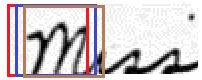
\includegraphics[width=0.19\textwidth]{images/sliding.jpg}
\caption{Overlapping windows 40 pixels wide, spaced 7 pixels}
\end{figure} 



While the simplest way to create the windows in the code would be simply cutting the original image in pieces through specialized functions of the \textit{Leptonica} library, these steps require a great amount of memory and time. We have thus preferred to increase the complexity of the functions that search for the features, to whom we pass as a variable the original images with information about the \textit{offset} at which to start the search and the \textit{width} of the window. The width of the window passed has actually a non banal meaning due to the fact that different features are associated with areas of the image with varying dimensions: for example it is not sensible to search for an horizontal line and a vertical line utilizing windows with the same width due to the fact that horizontal lines realistically will require windows with great width but will not have requisites on the height.


In particular, the features with less space requirements are searched in both 20 pixels halves of the windows and their strings are appended to the image string, the whole 40 pixels window is then searched for the space-hungry features, only then their identifiers are added to the general string. 

\begin{figure}[!htpb]
\centering
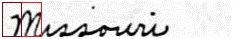
\includegraphics[width=0.35\textwidth]{images/missouri_windows.jpg}
\caption{A window and its first half}
\end{figure} 

The height of the windows used is never considered as a parameter since for all the features searching functions the height is customarily the height of the sample.  

\subsubsection{Whitespace}  

The first feature that is searched in the windows is the presence of white space. This way if a window is identified as blank there won't be a need to proceed with the search of the other features, saving time.

\begin{figure}[!htpb]
\centering
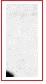
\includegraphics[width=0.06\textwidth]{images/whitespace.jpg}
\caption{A Whitespace}
\end{figure} 

A window is identified as blank if the average pixel values is below a pre-set threshold.

The string associated with the Whitespace is " ".
This string is not given much consideration when calculating distances since it may bring problems if images with the same word are not properly centered in the segmented samples, while differentiating words through the presence of spaces doesn't bring many fruits.

\subsubsection{Loop}

The feature that represents a loop requires the search of the whole 40 pixels window.
The localization of a loop starts from the search of a black pixel. The idea behind is that a point on the border of a loop is such that by looking in a decided direction (in this case the y axis) we meet two pixel's value transitions first from black to white and then from white to black. Between the two transitions for a loop to be recognised there must be a minimum number of white pixel, number that is decided discretionally in the code.

\begin{wrapfigure}{l}{0.3\textwidth}
  \vspace{-20pt}
  \begin{center}
    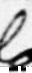
\includegraphics[width=0.06\textwidth]{images/loop.jpg}
  \end{center}
  \vspace{-20pt}
  \caption{A loop}
  \vspace{-10pt}
\end{wrapfigure}

To recognise a loop the above condition must also be verified in the other cardinal axis. To do so, starting from the center of the supposed loop (the median value of the segment described above) we check that moving either right or left we find a transition from white to black after a suitable number of white pixels.

The implemented method has numerous problems related to the difficulty of finding the best white spaces threshold: an excessively little minimum number of white pixels makes us recognise as loops white noise that happens while scanning images, a threshold too high forces us to discard some small but real loops. The method also does not take into account the thickness of the stroke, rendering the overall recognition harder, with appropriate threshold values tough we can achieve good results.

The string associated with the Loop feature is "LL".
\subsubsection{Dot}

\begin{wrapfigure}{r}{0.3\textwidth}
  \vspace{-20pt}
  \begin{center}
    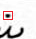
\includegraphics[width=0.06\textwidth]{images/dot}
  \end{center}
  \vspace{-20pt}
  \caption{A dot}
  \vspace{-10pt}
\end{wrapfigure}

To search for Dots within the segment we first proceed locating the \emph{connected components} inside of it. The individual components are extracted and inserted into a \emph{box} of which we know the size and the relative position to the segment.


At this point we search for those boxes with dimensions between two pre-set values (minimum and maximum radius), those that meet this condition are boxes that contain most likely points.
Using the connected components we can thus retrieve dots in a simple way.

The string associated with the Dot feature is ".....".

It is particularly long because the dot helps distinguish the words that contain the "i" letter and a dot is easily recognised with little error.

\subsubsection{Diagonal line}

The feature representing a diagonal line, both upward and downward facing, is extracted through a simple exhaustive scansion of the window for lines of connected black pixels that have an incline in a range of values and are sufficiently long.

In the case of an upward facing diagonal, given a black pixel we consider it connected to another black pixel if this second one is in one of 3 different position that are illustrated in Figure \ref{pixels}. The lines recognized are thus all those with gradient between 30 and 60\%.

\begin{figure}[!htpb]
\centering

\includegraphics[width=0.12\textwidth]{images/diagP.jpg}
\caption{Given the black pixel we search for other black pixels in the 3 positions, the red one is given priority}
\label{pixels}
\end{figure} 
\vspace{3mm}
At the moment the function doesn't account for the width of the lines found, thus diagonal features can be recognised in a formless blob of black pixels that is sufficiently big. 

\begin{figure}[!htpb]
 \centering
 \subfigure[]
   {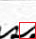
\includegraphics[width=0.07\textwidth]{images/diagonal.jpg}}
 \hspace{15mm}
 \subfigure[]
   {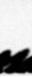
\includegraphics[width=0.046\textwidth]{images/blob.jpg}}
 \caption{proper Diagonal feature(a) and a formless blob that introduces errors(b), in this second both upward and downward diagonal lines are recognised}
  \end{figure}
\vspace{2mm}
   
A distinction in the associated string is introduced for the diagonal features that appear in the lower or upper bottom of the window, moreover the searches for the two kinds of lines are separate.
At most in a window the function identifies a couple of upward and a couple of downward facing lines (lower and upper parts), once one has been found it stops searching for the same type.
The lines that are found are further categorised on their length if medium or long.

Many different strings are associated with the Diagonal feature, they will be properly listed in the Table \ref{features}.
In particular the string associated with the "long" version of a feature is made from the "medium" version of the string at which is attached an other character: this allows to distinguish features based on their length while at the same time maintaining similarity with a shorter version of themselves to account for variation in the stroke used to write the same word.  
 
\subsubsection{Cross}
The function, having found at most a lower and upper case for upward and downward diagonal lines, proceeds to confront the edge points of these lines: if they possibly intersects it extracts a \emph{crossing} feature with distinction if the crossing happens in the lower or upper part of the window, priority is given to the bottom part if for example a bottom upward diagonal intersects an upper downward diagonal. 

The problems with this sub-feature are that intersections of bottom and upper lines of the same type (e.g. both upward facing) with different inclines are not recognised, in the same way there's no consideration for intersections made from lines that are not the "primary" bottom and upper diagonals: if in a single windows are present more lower upwards diagonals and one of them other than the first intersects the recognised downward diagonal, such a crossing is ignored.

\begin{wrapfigure}{l}{0.3\textwidth}
  \vspace{-20pt}
  \begin{center}
    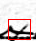
\includegraphics[width=0.06\textwidth]{images/cross.jpg}
  \end{center}
  \vspace{-20pt}
  \caption{A cross}
  \vspace{-10pt}
\end{wrapfigure}


The crossing feature may also not necessarily be a complete intersection, in fact for recognition there just needs to be a merging of a downward and upward line. 

The string associated depending if the cross is found in the upper or lower half is "X" and "x" respectively.
While it may seem that a crossing is distinctive of a word and thus deserving of more "characterizing force", that is the length of the associated strings, the difficulty in recognising the feature and it's uncertainty renders an excessive weight given to its presence dangerous for clustering purposes.
The feature is thus maintained for future improvements but doesn't bring immediate 
contributions to the application.

\subsubsection{Horizontal and Vertical line}
Both horizontal and vertical lines' features are extracted through
a simple scan of the window.

The horizontal lines requires a double-window for their implicit characteristic.
The function identifies a line if it finds a connected row or column of black pixels that has sufficient length, in particular it distinguishes the lines found in normal or long through an ulterior threshold.
In particular, as obvious difference from the diagonal line, no play is left to recognise inclined lines as horizontal or vertical.

Once a fitting line has been found the function keeps searching for more until the exhaustion of the allotted space. The scansion of the window is continued after having moved a certain distance from the last line found in order not to confuse a particularly thick stroke as different separate lines.
The corresponding string as thus no limitation in length other than the ones posed by the maximum number of lines that can fit in a window.

\begin{figure}[!htpb]
 \centering
 \subfigure[]
   {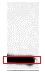
\includegraphics[width=0.07\textwidth]{images/hor.jpg}}
 \hspace{15mm}
 \subfigure[]
   {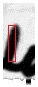
\includegraphics[width=0.05\textwidth]{images/ver.jpg}}
 \caption{Horizontal(a) and Vertical(b) features}
  \end{figure}
\vspace{2mm}

There still persists the problem that the stroke width is not fully considered so a big blob of black pixels is seen as a series of horizontal and vertical lines, at the same time such an occurrence is rare so the presence of many horizontal and vertical lines ends up distinguishing the word in itself.    

\subsubsection*{Recapitulation}
We present a recapitulation of the various features and their correspondent strings.
\begin{table}[!htbp]
\centering
\footnotesize
\begin{tabular}{|l | c |} 
 \hline  \multicolumn{1}{|p{2cm}|}{\bfseries Feature}
 & \multicolumn{1}{p{2cm}|}{\centering\bfseries Associated string} \\ [0.5ex] 
 \hline\hline
 Whitespace & " " \\ \hline
 Loop & "LL"\\\hline
 Dot & "....."\\ \hline
 Upward facing diagonal lower half, medium & "s" \\ \hline
 Upward facing diagonal lower half, long & "bs"  \\\hline
 Upward facing diagonal upper half, medium & "S" \\ \hline
 Upward facing diagonal upper half, long & "BS" \\\hline
 Downward facing diagonal lower half, medium& "u"\\ \hline
 Downward facing diagonal lower half, long &"vu" \\ \hline
 Downward facing diagonal upper half, medium& "U" \\\hline
 Downward facing diagonal upper half, long &"VU" \\\hline
 Cross upper & "X"\\\hline
 Cross lower & "x"\\\hline
 Horizontal line lower half, medium & "-"\\\hline
  Horizontal line lower half, long & "h-"\\\hline
   Horizontal line upper half, medium & "H-"\\\hline
    Horizontal line upper half, long & "Hh-"\\\hline
 Vertical line lower half, medium & "ii"\\\hline
  Vertical line lower half, long & "IIii"\\\hline
   Vertical line upper half, medium & "Vii"\\\hline
    Vertical line upper half, long & "VIIii"\\ 
 \hline
\end{tabular}
\caption{Recapitulation of the strings associated to each feature}
\label{features}
\end{table}



\subsection{Dimensional features}
While the already proposed structural features help in categorizing and recognising words to cluster, they aren't completely able to distinguish a word from similar others, we have thus searched for ways to improve the accuracy of the application:
while many optimizations have been added to the defined structural features we have found that adding another layer of features of a different kind, in this case \emph{dimensional}, helps greatly.
Moreover the complexity added is extremely limited: as can be seen later on in the Table \ref{table:2} the required calculation time doesn't increase in a particularly meaningful way: the majority of the process complexity isn't located in the features' extraction but rather in the clustering and construction of the LCS-distance matrix.  
Thus in order to improve word clustering we combine structural features with \emph{dimensional features} for each word, after constructing the distance matrices for both we combine them through a factor determined from testing. 

These dimensional features are exactly the ones previously utilized by our colleagues in the pre-existing work: height of the stroke, calculated through the difference between highest and lowest black pixel, and number of transition of the pixels' value from black to white and vice versa.

A simple explanation on how they are extracted can be found in section \ref{oldFeatures}.

\subsection{Features extraction example}

We present now an example of features extraction from a word sample, in this case it is presented an older implementation of our application but the ideas and process scheme are maintained constant.
In particular the older version was chosen to simplify the explanation since it uses smaller windows with lesser overlap so that it is visually more self-explanatory.

We initially create, as described in the section above, a sliding window that scrolls along the image by a fixed step. Then, for each section, we extract features and generate a substring.

\begin{figure}[!htpb]
\centering
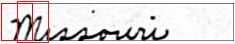
\includegraphics[width=0.5\textwidth]{images/missouri_crop.jpg}
\caption{Feature extraction from \emph{Missouri} word}
\end{figure} 

\begin{figure}[!htpb]
 \centering
 \subfigure[]
   {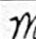
\includegraphics[width=0.06\textwidth]{images/missouri/0.jpg}}
 \subfigure[]
   {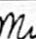
\includegraphics[width=0.06\textwidth]{images/missouri/1.jpg}}
 \subfigure[]
   {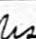
\includegraphics[width=0.06\textwidth]{images/missouri/2.jpg}}
 \subfigure[]
   {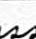
\includegraphics[width=0.06\textwidth]{images/missouri/3.jpg}}
 \subfigure[]
   {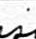
\includegraphics[width=0.06\textwidth]{images/missouri/4.jpg}}
 \subfigure[]
   {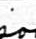
\includegraphics[width=0.06\textwidth]{images/missouri/5.jpg}}
 \subfigure[]
   {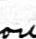
\includegraphics[width=0.06\textwidth]{images/missouri/6.jpg}}
 \subfigure[]
   {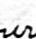
\includegraphics[width=0.06\textwidth]{images/missouri/7.jpg}}
 \subfigure[]
   {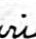
\includegraphics[width=0.06\textwidth]{images/missouri/8.jpg}}  
 \subfigure[]
   {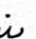
\includegraphics[width=0.06\textwidth]{images/missouri/9.jpg}}
 \subfigure[]
   {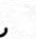
\includegraphics[width=0.06\textwidth]{images/missouri/10.jpg}}
 \subfigure[]
   {
\includegraphics[width=0.06\textwidth]{images/missouri/11.png}}
 \subfigure[]
   {
\includegraphics[width=0.06\textwidth]{images/missouri/12.png}}   
 \caption{Sliding window segmentation}
 \end{figure}

\begin{enumerate}[label=(\alph*)]
\item Some \textbf{diagonal lines} (ascending (s) and descending (u) ), at the top (S) and at the bottom (s) of the image. Generated string: ''\emph{sSUusSUSu}''.
\begin{figure}[!htpb]
\centering
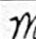
\includegraphics[width=0.06\textwidth]{images/missouri/0.jpg}
\end{figure} 
\item As the previous image and two more diagonal lines representing the "\emph{i}". An \textbf{horizonal line} (H). Generated string: ''\emph{sSUusSUSuHsu}''.
\begin{figure}[!htpb]
\centering
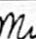
\includegraphics[width=0.06\textwidth]{images/missouri/1.jpg}
\end{figure} 
\item Some diagonal lines and, at the end of the window, an horizontal line. Generated string: ''\emph{ssSusSsH}''.
\begin{figure}[!htpb]
\centering
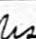
\includegraphics[width=0.06\textwidth]{images/missouri/2.jpg}
\end{figure} 
\item Two consecutive similar character represented by diagonal lines and \textbf{vertical lines} in the middle. Generated string: ''\emph{sVHsV}''.
\begin{figure}[!htpb]
\centering
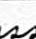
\includegraphics[width=0.06\textwidth]{images/missouri/3.jpg}
\end{figure} 
\item In that window we can find a \textbf{dot} (.). Generated string: ''\emph{ssVHs.}''
\begin{figure}[!htpb]
\centering
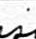
\includegraphics[width=0.06\textwidth]{images/missouri/4.jpg}
\end{figure} 
\item The same previous dot and a little \textbf{loop} (L) at the bottom. Generated string: ''\emph{ssVs.LssH}''.
\begin{figure}[!htpb]
\centering
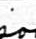
\includegraphics[width=0.06\textwidth]{images/missouri/5.jpg}
\end{figure} 
\item The same loop as previous, an horizontal line a vertical line and two diagonal. Generated string: ''\emph{LVHssu}''.
\begin{figure}[!htpb]
\centering
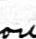
\includegraphics[width=0.06\textwidth]{images/missouri/6.jpg}
\end{figure} 
\item Generated string: ''\emph{ssVHus}''.
\begin{figure}[!htpb]
\centering
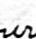
\includegraphics[width=0.06\textwidth]{images/missouri/7.jpg}
\end{figure} 
\item The other dot here. Generated string ''\emph{ssus.H}''.
\begin{figure}[!htpb]
\centering
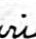
\includegraphics[width=0.06\textwidth]{images/missouri/8.jpg}
\end{figure} 
\item An i. Generated string: ''\emph{ssuu.}''.
\begin{figure}[!htpb]
\centering
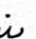
\includegraphics[width=0.06\textwidth]{images/missouri/9.jpg}
\end{figure} 
\item Only a diagonal line. Generated string: ''\emph{s}''.
\begin{figure}[!htpb]
\centering
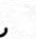
\includegraphics[width=0.06\textwidth]{images/missouri/10.jpg}
\end{figure} 
\item Empty window. Generated string: ''\emph{ }''.
\begin{figure}[!htpb]
\centering

\includegraphics[width=0.06\textwidth]{images/missouri/11.png}
\end{figure} 
\item Empty window. Generated string: ''\emph{ }''.
\begin{figure}[!htpb]
\centering

\includegraphics[width=0.06\textwidth]{images/missouri/12.png}
\end{figure} 
\end{enumerate}

Once those strings are generated they are combined together to generate the \textit{structure string} associated with the word sample. 

